\begin{comment}
\end{comment}

\chapter{Construction de codes correcteurs quantiques}

Dans le chapitre précédent, 
je me suis intéressé à la correction des erreurs lors de la communication classique.
Pour la suite de la thèse,
je quitterai ce régime pour m'intéresser au régime quantique.
Dans ce chapitre, 
je m'intéresserai plus particulièrement à la protection de l'information 
dans un modèle quantique simplifié avant de présenter la conception d'une mémoire 
quantique au prochain chapitre.
Ce modèle simplifié ressemble au canal binaire symétrique présenté au premier chapitre
et il permet d'étudier la construction de codes correcteurs d'erreurs quantiques sans prendre en compte les détails d'implémentation.

De façon semblable au scénario classique,
concevoir des codes correcteurs qui permettent de bien protéger l'information avec un nombre raisonnable de qubits supplémentaires est crucial.
En fait,
la présence des erreurs est l'un des obstacles parmi les plus
limitants pour la réalisation de calculs quantiques.
Ainsi, 
la correction d'erreurs ne se limite pas à des scénarios de communication 
comme dans le cas classique,
mais sera omniprésente dans un système de calcul quantique.

Cette importance accrue des erreurs dans les systèmes quantiques s'explique
principalement du fait qu'il s'agit de systèmes analogues plutôt que digitaux.
Un système est digital lorsque chacun de ses éléments peut prendre un nombre fini
de valeurs. 
Dans le cas des ordinateurs classiques,
chaque bit prend soit la valeur 0 ou la valeur 1.
Ainsi,
une quantité continue comme une différence de potentiel représente physiquement un bit tout en le protégeant des erreurs.
Par exemple,
le bit 0 peut être associé à une valeur de 0 volt et le bit 1 à une valeur de 5 volts.
Dans le cas où une valeur de 4.9 volts serait mesurée, il est fort probable que 
la valeur désirée était le bit 1.
Donc, en absence des perturbations externes présentent lors de la communication,
l'information classique est relativement robuste.

Au contraire, un système quantique est analogue puisqu'il existe une infinité d'états accessibles.
Par exemple, toutes paires de nombres complexes $a$ et $b$ telles que $a^2 + b^2 = 1$
représentent l'état d'un qubit.
Ainsi, 
une faible variation de ces paramètres représente un état différent
et distinguer l'état désiré d'un état corrompu est généralement impossible.
De plus, l'accumulation de ces petites différences peut complètement
changer le résultat d'un calcul.

Ces erreurs émergent généralement de processus de décohérence.
Par exemple,
un système quantique dans un état excité tend naturellement à retourner dans un état de moindre énergie.
Au milieu des années 1990,
plusieurs scientifiques croyaient que
les erreurs engendrées par la décohérence des systèmes quantiques
représentaient un obstacle insurmontable au calcul quantique~\cite{unruh_maintaining_1995, palma_quantum_1996, landauer_is_1995, chuang_quantum_1995}.
Leurs arguments reposaient entre autres sur le théorème de non-clonage~\cite{wootters_single_1982}
stipulant qu'il est impossible de copier l'état d'un qubit vers un second qubit.
Cela semblait donc empêcher l'utilisation de la redondance pour 
protéger le système des erreurs comme c'est le cas pour la communication classique.

Nous savons aujourd'hui comment contourner ces limitations. 
Les premiers à avoir proposé une solution sont Calderbank, Shor et Steane~\cite{calderbank_good_1996, steane_multiple-particle_nodate}.
D'ailleurs, à la prochaine section,
je vais introduire une importante famille de codes correcteurs quantiques, les codes CSS, qui porte leur nom.
En réponse à ce résultat, Gottesman~\cite{gottesman_stabilizer_1997} a introduit le formalisme des codes stabilisateurs
que je vais utiliser dans ce chapitre pour décrire les codes correcteurs quantiques.

Depuis,
plusieurs familles de codes correcteurs quantiques ont été introduites.
Les codes les plus étudiés sont sans aucun doute les codes de surfaces et 
les codes toriques introduits par Kitaev~\cite{kitaev_fault-tolerant_2003}.
Cependant,
ces codes, bien qu'excellent pour protéger le système,
ne permettent pas d'encoder efficacement un grand nombre de qubits~\cite{bravyi_tradeoffs_2010}.
Pour contrer ce problème,
les codes quantiques d'opérateurs de parité à faible 
densité~(LDPC, de l'anglais \textit{low-density parity-check})
reçoivent de plus en plus d'attention.
Cet intérêt est en partie stimuler par le succès des codes LDPC classiques introduits
par Gallager~\cite{gallager_low-density_1962}.
De plus, il a été montré par Gottesman~\cite{gottesman_fault-tolerant_2013}
qu'il est possible d'utiliser des codes quantiques LDPC pour 
construire des ordinateurs quantiques protégés des erreurs avec 
un surcout constant en qubits.
Il s'agit donc d'outils importants pour la réalisation du calcul quantique à grande échelle.

Les codes quantiques LDPC incluent plusieurs familles,
dont les codes par produit d'hypergraphes~\cite{tillich_quantum_2014}
et les codes par produit homologique~\cite{bravyi_homological_2014}.
Comme l'indique le nom de ces exemples,
les codes quantiques LDPC sont généralement obtenus par le produit 
de structures associées à des codes correcteurs classiques.
Dans le cadre de cette thèse,
j'ai conçu une approche qui permet plutôt de générer des codes correcteurs quantiques
directement,
sans avoir recours à une construction classique au préalable.
L'un des principaux avantages de cette méthode est sa flexibilité 
lors de la construction des codes.
En fait,
cette construction permet de générer n'importe quelle famille de codes stabilisateurs,
dont les codes LDPC.

Cette approche repose sur la résolution d'un problème de satisfaction de contraintes.
Bien que ce problème soit généralement difficile à résoudre,
j'ai numériquement identifié des régimes pour lesquels il est aisé de
construire des codes correcteurs quantiques
et des régimes pour lesquels la tâche est beaucoup plus ardue.
Cela, bien que surprenant, est un comportement attendu pour ce type de problème.

Je reviendrai sur cela après avoir présenté le formaliste des canaux bruités quantiques 
et des codes stabilisateurs.
Finalement,
je présenterai l'article expliquant la construction et 
mettant de l'avant les résultats de ce projet.

\section{Correction d'erreurs quantique}

\subsection{Canaux bruités quantiques}

Un état quantique est généralement représenté par un opérateur de densité $\rho$
de trace unité.
Une évolution arbitraire d'un état $\rho$ vers un état $\rho'$
c'est-à-dire une combinaison d'opérations unitaires,
de mesures et d'interactions avec l'environnement, 
est représentée par une application
\begin{align}
  \rho' = \mathcal{E}(\rho).
\end{align}
Pour décrire plus précisément cette transformation,
j'utiliserai les opérateurs de Krauss.
Dans ce cas,
l'application est définie par
\begin{align}
  \mathcal{E}(\rho) = \sum_{k} E_k \rho E_k^\dag,
\end{align}
avec la condition que 
\begin{align}
  \sum_k E_k^\dag E_k = I.
\end{align}
Cette dernière permet d'assurer que $\tr(\mathcal{E}(\rho)) = 1$.

Dans leur excellent livre d'introduction à l'informatique quantique de 
Neilsen et Chuang~\cite{nielsen_quantum_2010} motivent en détail 
cette définition générale pour l'évolution d'un état quantique.
Ainsi, je me limite à une justification intuitive de cette définition
et j'invite les personnes intéressées à consulter le huitième chapitre de ce livre.

De façon générale,
l'état $\rho$ évolue au sein d'un environnement dont les états de base 
sont $\qty{\ket{e_0}, \ket{e_1}, \ldots}$.
Au début d'une expérience (ou d'un calcul),
le système et l'environnement sont dans un état de produit tensoriel,
soit un état sans intrication.
De plus, il est suffisant de considérer que l'environnement est dans l'état 
pur $\ket{e_0}$.
En effet,
si ce n'est pas le cas, il suffit de choisir un environnement plus grand jusqu'à 
obtenir un état pur.
Ainsi,
l'état initial du système et de l'environnement est $\rho \otimes \op{e_0}$.

\begin{figure}
  \begin{center}
    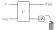
\includegraphics{figures/circuit_canal_quantique.pdf}
  \end{center}
  \caption[Représentation en circuit d'un canal quantique]{
    Représentation en circuit d'un canal quantique.
    Le résultat de la mesure est ignoré.
  }
  \label{fig:circuit_canal_quantique}
\end{figure}

Par la suite,
un opérateur unitaire $U$ est appliqué sur le système et l'environnement,
suivi d'une mesure de l'environnement sans connaitre le résultat.
Le circuit correspondant est illustré à la figure~\ref{fig:circuit_canal_quantique}.
Ainsi, l'état final du système est
\begin{equation}
  \mathcal{E}(\rho) 
  = \tr_{\text{env}}\qty(U(\rho \otimes \op{e_0})U^\dag)
  = \sum_k \bra{e_k}U(\rho \otimes \op{e_0}) U^\dag \ket{e_k}
  = \sum_k E_k \rho E_k^\dag
\end{equation}
avec $E_k = \mel{e_k}{U}{e_0}$.
Alors,
l'application $\mathcal{E}$ représente la transformation de l'état d'un système quantique
lorsque celui-ci interagit avec son environnement et que l'on ignore l'état final
de l'environnement.

Une autre interprétation est qu'à la suite de l'application $\mathcal E$,
le système se retrouve dans l'état $\rho_k \propto E_k \rho E_k^\dag$
avec probabilité $p_k = \tr(E_k \rho E_k^\dag)$.
Il est alors possible d'écrire l'application selon
\begin{align}
  \mathcal E(\rho) = \sum_k p_k \rho_k.
\end{align}
Cette formulation montre clairement l'utilité de $\mathcal E$ pour
représenter un canal bruité quantique.
De façon comparable au canal bruité classique,
un canal quantique transforme un premier état 
vers un second état choisi aléatoirement.

Dans cette thèse,
je me limite aux canaux bruités quantiques avec des opérateurs 
de Krauss $E_k$ proportionnels aux opérateurs de Pauli.
Les opérateurs de Pauli pour un seul qubit sont 
\begin{align}
  &I = \op{0}{0} + \op{1}{1}, 
  &&Y = -i\op{0}{1} + i\op{1}{0}, \notag \\
  &X = \op{0}{1} + \op{1}{0}, 
  &&Z = \op{0}{0} - \op{1}{1}.
\end{align}
Le groupe~\footnote{Je fais un rappel des notions de théorie des groupes à l'annexe~\ref{chap:theo_groupes}}
de Pauli $\mathcal P_n$ de $n$ qubits est un groupe multiplicatif sur 
l'ensemble des opérateurs $\qty{I, X, Y, Z}^n$ avec une phase parmi $\qty{1, i, -1, -i}$.
Dans ce cas,
le canal s'écrit généralement comme
\begin{align}
  \mathcal E(\rho) = \sum_{P \in \mathcal P_n} p_P P\rho P.
\end{align}
Le poids $|P|$ d'un opérateur de Pauli $P$ est le nombre d'opérateurs différent de $I$ qui le compose.
Par exemple, $|i\cdot XIYX| = 3$.
Pour l'ensemble des canaux que je considèrerai,
la probabilité d'une erreur $P \in \mathcal P_n$ diminue exponentiellement avec le poids 
de celle-ci.

De prime abord,
cette approche semble limitée,
mais puisque les opérateurs de Pauli forment une base,
il est possible de représenter un opérateur de Krauss
comme une combinaison linéaire de ces derniers.
Ainsi,
un protocole qui permet de protéger un système quantique contre les erreurs 
$Q \subseteq \mathcal P_n$ protège également le système contre toutes les 
combinaisons linéaires des opérateurs de $Q$~\cite{knill_theory_1997}.
Ce modèle est donc suffisant pour construire une théorie générale de la correction d'erreurs quantique.

En particulier,
dans l'article de ce chapitre,
j'utilise le canal d'effacement quantique pour évaluer la performance
des codes correcteurs que je construis.
Ce canal représente la situation où l'information contenue dans certains qubits,
dont on connait la position, est complètement perdue.
On dit alors que ces qubits sont effacés.
En laboratoire, cela correspond par exemple à la défaillance d'une composante électronique
ou à la perte d'un photon.
Pour représenter cette situation, l'état $\rho$ est associé à un second registre
permettant de marquer les qubits effacés.
Dans le cas d'un seul qubit avec une probabilité d'effacement $p$,
le canal s'écrit
\begin{equation}
  \mathcal E_p(\rho \times \op{0}) 
  = (1 - p) \rho \otimes \op{0} + p \frac{I}{2} \otimes \op{1}.
\end{equation}
Dans cet équation,
l'opérateur $I/2$ est utilisé pour représenter un état maximalement mixé
sans aucune information sur l'état initial $\rho$.
Le second registre indique la présence de l'effacement.
Comme 
\begin{align}
  I = \frac{1}{2} \qty(
  I\rho I + X \rho X + Y \rho Y + Z \rho Z
)
\end{align}
pour tout opérateur $\rho$\footnote{
  En notant $f(\rho) = I\rho I + X\rho X + Y \rho Y + Z \rho Z$,
  on remarque que $f(I/2) = I$ et que $f(X) = f(Y) = f(Z) = 0$.
  De plus,
  pour avoir une trace unité,
  une matrice densité se décompose comme $\rho = I/2 + aX + bY + cZ$,
  ce qui permet de conclure.
},
il est possible de réécrire le canal à l'aide d'opérateurs de Pauli à 2 qubits.
Ainsi,
\begin{equation}
  \mathcal E_p(\rho \times \op{0}) 
  = \qty(1 -  p) \rho \otimes \op{0} + \frac{p}{4} \qty(\rho + X \rho X + Y \rho Y + Z \rho Z)\otimes \qty(X\op{0}X).
\end{equation}

Dans l'article,
je présente plus en détail le canal d'effacement.
Entre autres,
je généralise le canal au cas à plusieurs qubits
en plus de présenter un algorithme de décodage optimal applicable à n'importe quel
code correcteur quantique pour ce canal.
Ce décodeur universel est la raison principale pour utiliser le canal d'effacement.
Celui-ci permet d'étudier de nouveaux codes sans nécessairement avoir besoin de construire des 
décodeurs spécialisés pour des canaux bruités plus complexes~(voir par exemple \cite{pastawski_holographic_2015, gullans_quantum_2021}).

Dans le chapitre suivant,
j'utiliserai un modèle de bruit plus réaliste qui permet
de représenter une mémoire quantique.
Celui-ci est également construit à partir d'opérateurs de Krauss proportionnels à des
opérateurs de Pauli.

\subsection{Codes stabilisateurs}

L'une des meilleures ressources pour une présentation complète du formalisme des codes
stabilisateurs est la thèse de doctorat de Gottesman~\cite{gottesman_stabilizer_1997}.
Dans cette section,
je me limiterai plutôt aux concepts essentiels à la compréhension des travaux et de l'article.

De façon comparable aux codes classiques,
les codes correcteurs quantiques encodent les états d'un espace de Hilbert
dans un sous-espace d'un espace de plus grande dimension.
Dans le cas des qubits,
les états de l'espace de Hilbert $\mathcal H_2^k$ sont encodés à l'aide d'un
sous-espace $\code \subseteq \mathcal H_2^n$.
Pour préserver la linéarité de la mécanique quantique,
le code $\code$ doit être un espace linéaire.
Ainsi,
si $\ket\psi, \ket\phi \in \code$,
alors $\alpha\ket\psi + \beta\ket\phi \in \code$ 
pour toutes paires $\alpha, \beta$ de nombres complexes.~\footnote{
  Pour simplifier la présentation,
  je laisse tomber la normalisation des états quantiques.
}

Un exemple de code quantique permettant d'encoder un qubit à l'aide de neuf qubits est 
le code de Shor~\cite{shor_scheme_1995} défini par l'encodage
\begin{align}
  \ket{0} \to \ket{\bar{0}} = (\ket{000} + \ket{111}) \otimes (\ket{000} + \ket{111}) \otimes (\ket{000} + \ket{111}), \notag \\
  \ket{1} \to \ket{\bar{1}} = (\ket{000} - \ket{111}) \otimes (\ket{000} - \ket{111}) \otimes (\ket{000} - \ket{111}).
  \label{eq:code_shor}
\end{align}
Par linéarité, l'état $\alpha \ket{0} + \beta \ket{1}$ est encodé avec l'état 
$\alpha \ket{\bar{0}} + \beta\ket{\bar {1}}$.
Je ne détaillerai pas ce code,
mais celui-ci illustre qu'il n'est pas pratique d'énumérer l'encodage des états de base
pour définir un code.
D'abord,
l'espace $\mathcal H_2^k$ requiert $2^k$ états de base
et chacun de ceux-ci implique une superposition de $\mathcal O(2^n)$ 
si le code $\code$ est un sous-espace de l'espace de Hilbert à $n$ qubits.

Le formalisme des stabilisateurs permet de contourner ce problème en offrant une 
représentation beaucoup plus efficiente de certains états quantiques.
D'abord,
un état $\ket\phi$ est stabilisé par l'opérateur $U$ lorsque $U\ket\psi = \ket\psi$,
soit lorsque $\ket \phi$ est un état propre de valeur propre $+1$ de $U$.
Un état ou un sous-espace est alors représenté par les opérateurs qui le stabilisent.
Par exemple,
l'état $\ket{00} + \ket{11}$ est l'unique état à deux qubits stabilisé par 
les opérateurs $XX$ et $ZZ$. 
De même,
les états $\ket 00$ et $\ket 11$ forment une base
pour les états stabilisés par l'opérateur $ZZ$.
Il est important de choisir des opérateurs qui commutent pour assurer 
que ceux-ci partagent les mêmes états propres.
De plus, l'opérateur identité $I$ stabilise tous les états
et l'opérateur $-I$ ne stabilise aucun état.

De façon plus générale,
un groupe stabilisateur $\mathcal S$ pour $n$ qubits est un sous-groupe abélien 
du groupe de Pauli $\mathcal P_n$ excluant l'opérateur $-I$.
Cette exclusion implique également que tous les opérateurs ayant la phase $i$ ou $-i$ sont exclus.
Un code stabilisateur $\code(\mathcal S)$ est alors l'espace des états stabilisés par $\mathcal S$.
De plus,
puisque les états stabilisés par les opérateurs $P, Q \in \mathcal P_n$ sont également
stabilisés par l'opérateur $PQ$,
il est commun de choisir un ensemble de générateurs $g(\mathcal S) = \qty{S_1, \ldots, S_m}$
pour décrire le groupe stabilisateur
\begin{align}
  \mathcal S = 
  \qty{
    \prod_{i=1}^m S_i^{a_i} : \vb a \in \qty{0, 1}^m
  }
\end{align}
de $2^m$ éléments.
Lorsque les générateurs sont indépendants,
c'est-à-dire qu'il n'est pas possible d'en obtenir un comme le produit des autres,
le code $\code(\mathcal S)$ a une dimension $2^{n - m}$.
Ainsi, 
pour encoder $k$ qubits avec un code de $n$ qubits,
exactement $m = n - k$ générateurs indépendants sont nécessaires.

Le code de Shor introduit à l'équation~\eqref{eq:code_shor} est stabilisé
par le groupe généré par les opérateurs 
\begin{gather}
    X_1 X_2 X_3 X_4 X_5 X_6, \quad
    Z_1 Z_2, \quad Z_4 Z_5, \quad Z_7 Z_8, \notag \\
    X_4 X_5 X_6 X_7 X_8 X_9, \quad
    Z_2 Z_3, \quad Z_5 Z_6, \quad Z_8 Z_9.
\end{gather}
Dans ce cas précis,
le formalisme stabilisateur peut sembler légèrement encombrant,
mais il permet généralement de représenter un code de $n$ qubits encodant $k$ qubits
à l'aide de $n - k$ opérateurs de poids $\mathcal O(n)$.
Le cout total de la représentation est alors $\mathcal O(n^2)$, ce qui est un gain exponentiel
par rapport à l'énumération des états de base du code en notation de Dirac.
Pour la suite,
j'utiliserai la notation $[n, k]$ pour représenter un code stabilisateur arbitraire 
encodant l'espace $\mathcal H_2^k$ dans un sous-ensemble $\code \subseteq \mathcal H_2^n$.

Le syndrome d'une erreur $E \in \mathcal P_n$,
qui affectent un état $\ket\psi$ quelconque d'un code $[n, k]$,
est le résultat des mesures des générateurs du groupe stabilisateur.
Puisque les opérateurs de Pauli commutent ou anticommutent,
le résultat de chacune de ces mesures est $+1$ ou $-1$.
En effet, si $SE = \pm ES$ pour un stabilisateur $S$,
alors
\begin{equation}
  SE\ket\psi = \pm E S \ket\psi = \pm E\ket\psi.
\end{equation}
Ainsi,
l'état $E\ket\psi$ est un état propre de valeur propre $\pm 1$ de $S$.
Les composantes du syndrome $\vb{s}(E) \in \qty{+1, -1}^{n - k}$
sont données par la relation $S_iE = s_i S_i E$ pour $S_i \in g(\mathcal S)$.

Il est important de noter que le syndrome est indépendant de l'état $\ket \psi$.
Conséquemment,
une mesure du syndrome permet de détecter la présence d'erreurs sans corrompre l'état du système.
À partir de cette information,
un décodeur essaie de trouver une correction $F$ telle que $FE \in \mathcal S$, 
soit que $FE\ket\psi = \ket\psi$ pour tout état code $\ket\psi$.
Le choix de la correction n'est pas unique, car, si $FE \in \mathcal S$,
alors $(SF)E \in \mathcal S$ pour tous $S \in \mathcal S$.
Ainsi,
toutes corrections $F' = SF$ sont également valides.

Formellement,
tous les opérateurs $P \in \mathcal P_n$ de la même classe du groupe quotient $\mathcal P_n/\mathcal S$
ont le même effet sur le code puisque $P\ket\psi = PS\ket\psi$ pour tout $S \in \mathcal S$.
La classe d'un opérateur $P \in \mathcal P_n$ est l'ensemble $P\cdot \mathcal S = \qty{PS : S\in \mathcal S}$,
soit l'ensemble des opérateurs équivalent après multiplication par un stabilisateur.
De plus,
comme $|\mathcal P_n| = 4^{n+1}$,
le groupe quotient $\mathcal P_n/\mathcal S$ d'un code $[n, k]$ tel que $|\mathcal S| = 2^{n - k}$
possède $2^{n+k+2}$ classes.
En comparaison,
seulement $2^{n-k}$ syndromes sont possibles,
ce qui implique que $2^{2k + 2} = 4^{k + 1}$ classes d'opérateurs ont exactement le même syndrome,
mais des effets différents sur le code.

Les opérateurs appartenant aux classes ayant le syndrome $\qty{+1, +1, \ldots, +1}$
sont des représentations à $n$ qubit des opérateurs de Pauli $\mathcal P_k$
agissant sur le code.
Ces opérateurs forment le groupe des opérateurs logiques $\mathcal L$ et correspondent
au centralisateur,
\begin{align}
  C_{\mathcal P_n}(\mathcal S) 
  = \qty{P \in \mathcal P_n : PS = SP, \forall S \in \mathcal S},
\end{align}
du groupe stabilisateur.
Puisqu'un opérateur logique $L \in \mathcal L$ commute avec l'ensemble des stabilisateurs,
\begin{equation}
  S(L\ket\psi) = LS\ket\psi = L\ket\psi
\end{equation}
pour tout état code.
En conséquence,
$L\ket\psi$ est également un état code.
De façon similaire,
pour un syndrome arbitraire,
les $4^{k+1}$ classes ayant ce syndrome sont reliées par les opérateurs logiques.

On remarque que $\mathcal S \subset \mathcal L$.
En effet, le groupe stabilisateur correspond à l'opérateur $I$ sur le code.
De même, les classes $-\mathcal S$, $i\mathcal S$ et $-i\mathcal S$ correpondent
aux opérateurs $-I$, $iI$ et $-iI$.
La correspondance entre les autres opérateurs logiques et opérateurs de Pauli est
arbitraire tant que les relations de commutations sont respectées.

La conséquence de tout cela est qu'il est possible de décomposer un opérateur
$E \in \mathcal P_n$ en produit $LC$ où $C$ est un opérateur de même syndrome que $E$
et $L$ est un opérateur logique.
Il n'est pas nécessaire que $E = LC$, mais plutôt que $LC$ soit un élément de la classe $E \cdot \mathcal S$.
Cette décomposition permet de construire une procédure de décodage optimale que l'on 
nomme décodeur par maximum de vraissemblance (MV).
À partir du syndrome de l'opérateur $E$, 
le décodeur MV choisi d'abord aléatoirement une correction $C$ de même syndrome avant
de choisir un opérateur logique selon
\begin{align}
  L_{\text{MV}} = \arg\max_{L \in \mathcal L} \sum_{S \in \mathcal S} \Pr[LSC].
\end{align}
L'idée derrière le décodeur MV est qu'il existe un opérateur logique $L^*$ tel que $C = L^*E$.
Alors, le décodage est un succès si $L_{MV}$ et $L^*$ ont la même classe,
c'est-à-dire si $L_{MV}C = SE$ pour un certain stabilisateur $S \in \mathcal S$.
Ainsi, pour tout opérateur logique $L$, nous avons que 
\begin{align}
  \sum_{S\in \mathcal S} \Pr[LSC]
  =
  \sum_{S\in \mathcal S} \Pr[LSL^*E]
  =
  \sum_{S\in \mathcal S} \Pr[LL^*SE].
\end{align}
Dans le cas typique,
le poids de $E$ est faible puisque la probabilité d'un opérateur diminue avec son poid.
Ainsi, la somme est maximisée par $LL^* \in \mathcal S$ si le poids de chacun des opérateurs de
$\mathcal L \setminus \mathcal S$ est élevé.
Sinon,
la somme est maximisée par $LL^* \equiv P \in \mathcal L \setminus \mathcal S$ 
et l'application de cette correction laisse le système avec une erreur $L_{MV}CE = LL^*EE = P$ indectable.

Le décodeur échoue dans deux cas,
soit si le poids de $E$ est élevé, ce qui est hors de notre contrôle,
ou s'il existe un opérateur logique non stabilisateur de faible poids.
Ainsi,
il est important de construire des codes stabilisateurs pour lesquels la distance minimale,
\begin{align}
  d = \min_{L \in \mathcal L \setminus \mathcal S} |L|,
\end{align}
est élevée.
Le décodeur MV permet de corriger toutes les erreurs dont le poids est inférieur à $d / 2$.
Il n'est pas exclus que des erreurs de poids plus élevés soit corrigibles, 
mais les paramètres $n$, $k$ et $d$ d'un code permettent d'estimer rapidement la capacité
de ce dernier à corriger les erreurs en fonction de son rendement $k/n$.

Par contre,
calculer la distance minimale d'un code requiert de comparer le poid d'un nombre exponentiel d'opérateurs.
Il en est de même pour le calcul de $L_{MV}$ qui requiert un nombre exponentiel de compaisons.
Il est donc généralement impossible de calculer ces quantité et des simulations numériques 
doivent être effectuées pour estimer la performance d'un code à l'aide d'un décodeur sous-optimal.
Je reviendrai sur ce point à la section~\ref{sec:seuil_perf} après avoir présenté
les codes de Calderbank-Shor-Steane et une représentation graphique des codes
stabilisateurs aux prochaines sections.

\subsection{Codes CSS}

\subsection{Graphes de Tanner}


\subsection{Théorème du seuil et évaluation de la performance des codes correcteurs quantiques}
\label{sec:seuil_perf}
CITER Gottesman-Knill



\section{Problèmes de satisfaction de contraintes}
\subsection{Transition de phases et seuil de satisfiabilité}

\section{Article : Une multitude de codes stabilisateurs éparses}

Cet article soumis au journal Quantum à l'été 2022 a pour titre original
\textit{Finite-rate quantum sparse codes aplenty}.
Celui-ci était toujours en processus de révision lors de la soumission de cette thèse.

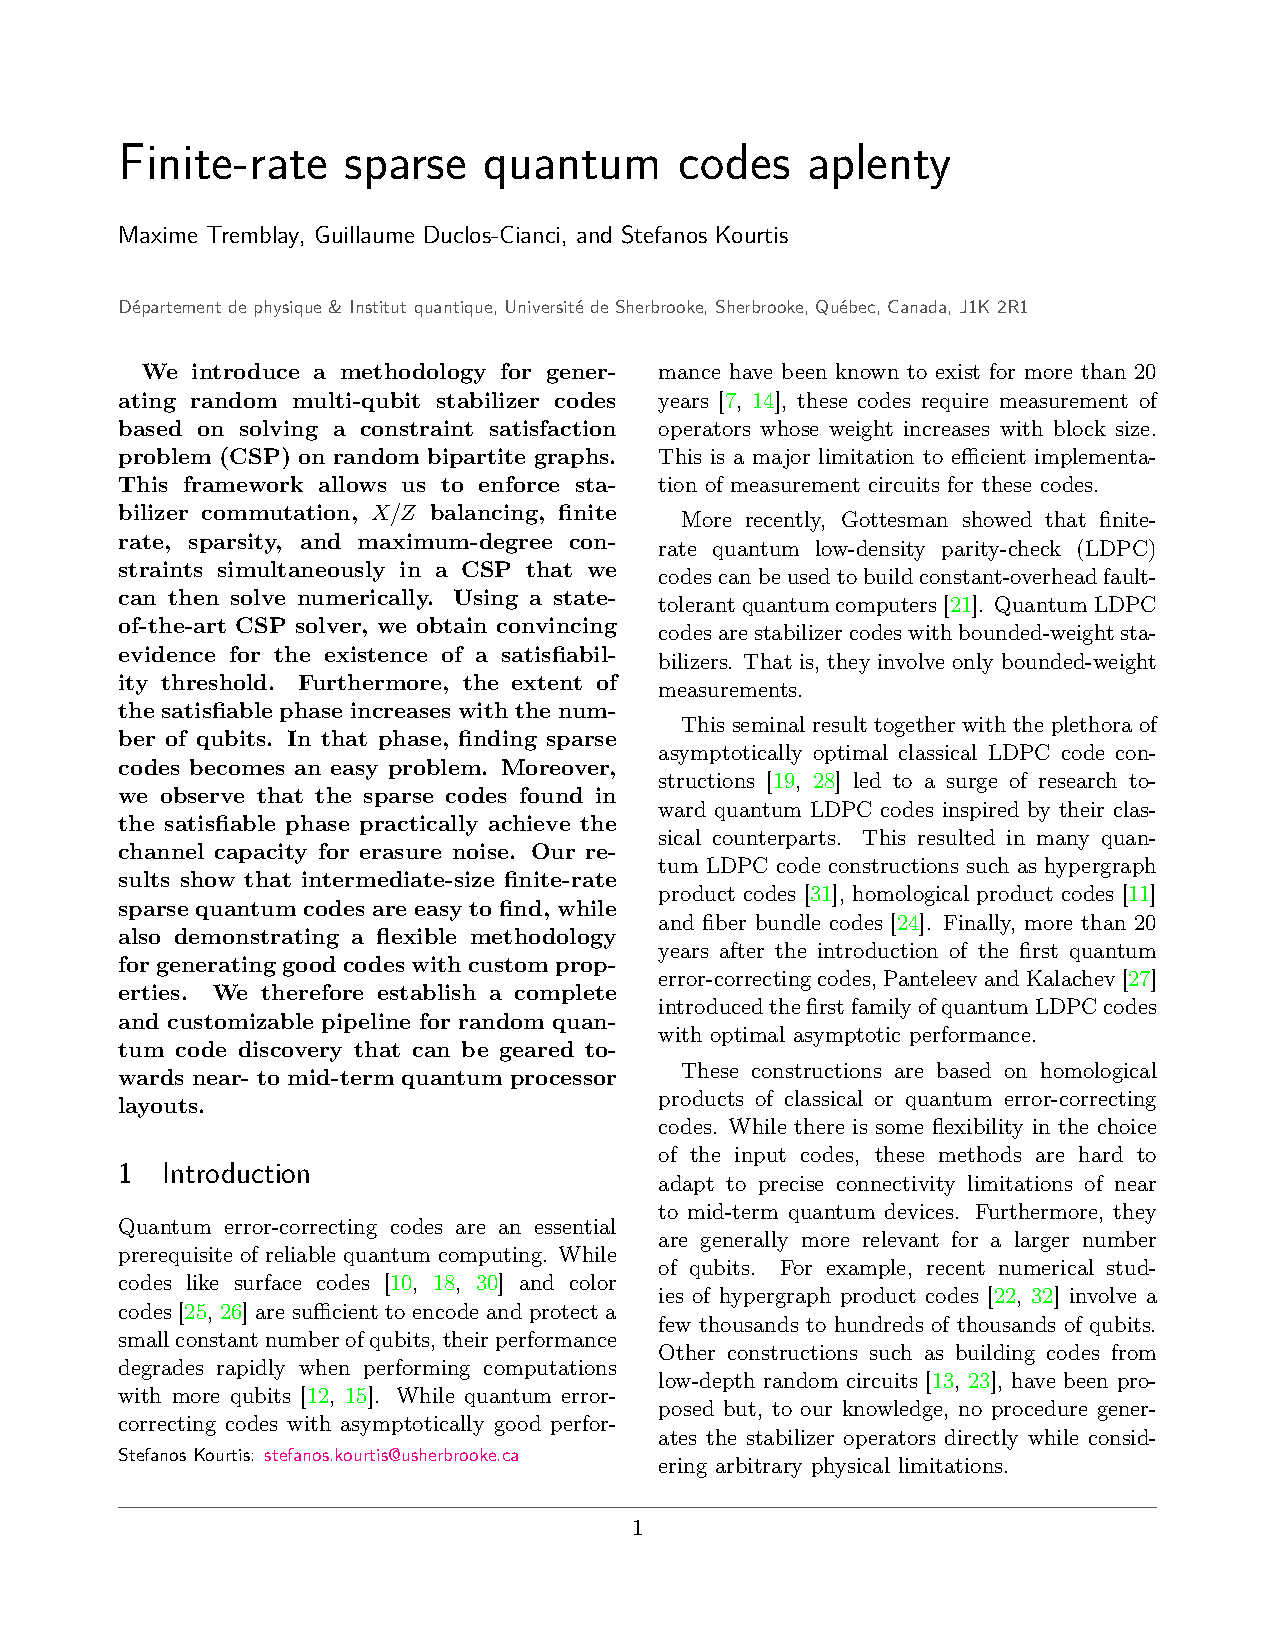
\includepdf[pages=-]{articles/sat_codes_construction.pdf}
